\documentclass[17pt,sans,mathserif]{beamer}

\setbeamertemplate{navigation symbols}{}

\setbeamercolor{background canvas}{bg=white}
\setbeamercolor{normal text}{fg=black}
\setbeamercolor{itemize item}{fg=red!80!black}
\setbeamercolor{frametitle}{fg=red!80!black}

\setbeamercolor{what how where}{bg=black,fg=gray!10!white}

\usepackage[absolute,overlay]{textpos}
\setlength{\TPHorizModule}{1pt}
\setlength{\TPVertModule}{1pt}


\usepackage{sgamevar}


\newcommand{\whw}[1]{
{
  \usebeamercolor[fg]{what how where}
  \setbeamercolor{background canvas}{bg=what how where.bg}
  \begin{frame}
    \begin{center}
      \Huge
      \textbf{#1}
    \end{center}
  \end{frame}
}
}

\usepackage{tikz}
\usetikzlibrary{shapes,arrows}
\usetikzlibrary{positioning}
\tikzstyle{block} = [draw, rectangle, minimum size=1cm]
\tikzstyle{sum} = [draw, circle, node distance=2cm]
\tikzstyle{input} = [coordinate]
\tikzstyle{output} = [coordinate]
\tikzstyle{pinstyle} = [pin edge={to-,thick,black}]

\begin{document}

{
  \usebackgroundtemplate{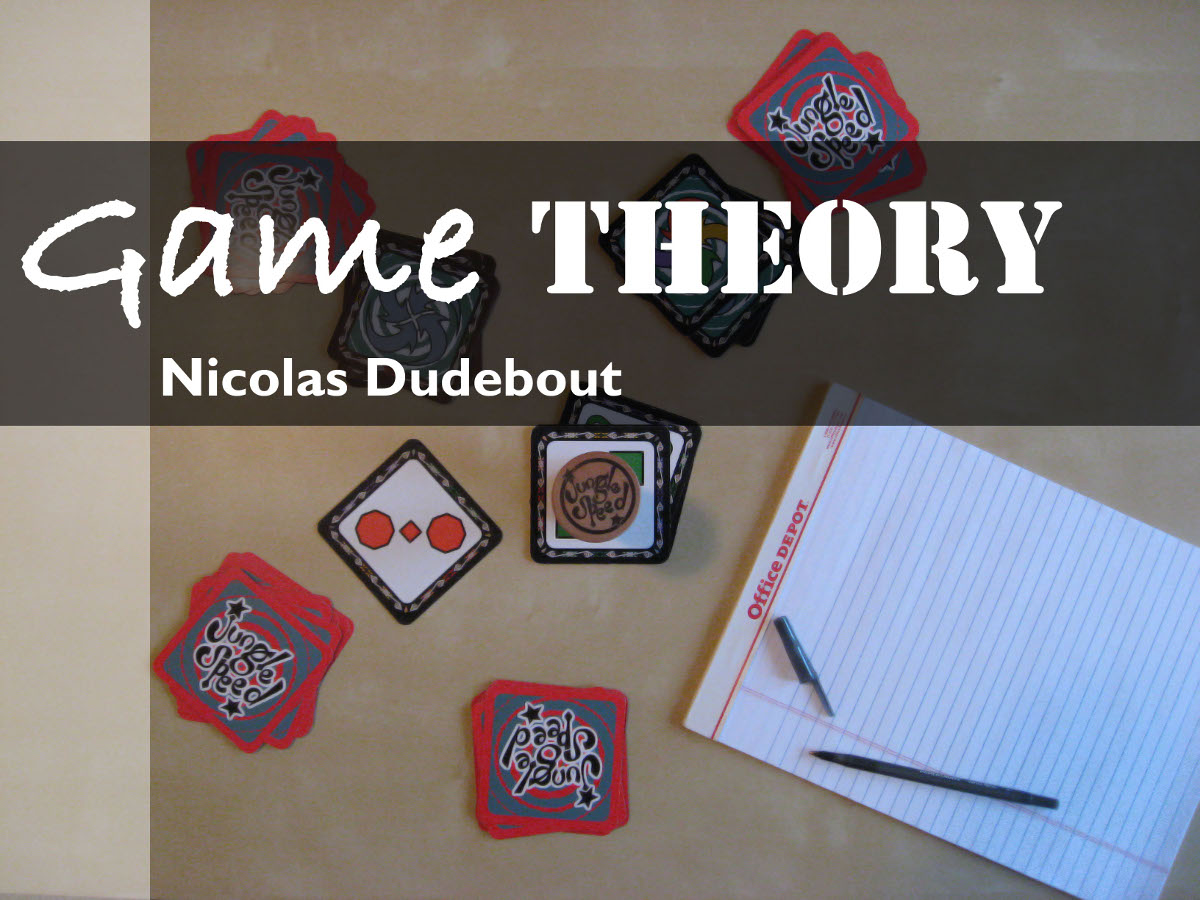
\includegraphics[width=\paperwidth,height=\paperheight]{images/game_theory.jpg}}
  \begin{frame}
  \end{frame}
}

\tikzstyle{whitestripe}=[draw=white, fill=white, fill opacity=0.7,rectangle,
inner sep=15pt, inner xsep=400pt]

\tikzstyle{blackstripe}=[draw=white, fill=white, fill opacity=0.7,rectangle,
inner sep=15pt, inner xsep=400pt]


{
  \usebeamercolor[fg]{what how where}
  \setbeamercolor{background canvas}{bg=what how where.bg}
  \begin{frame}

    {\Large \textbf{What}} is game theory?
    \bigskip

    \pause
    {\Large \textbf{How}} do we study it?
    \bigskip

    \pause
    {\Large \textbf{Where}} is research headed?
  \end{frame}
}

\whw{What?}

{
  \usebackgroundtemplate{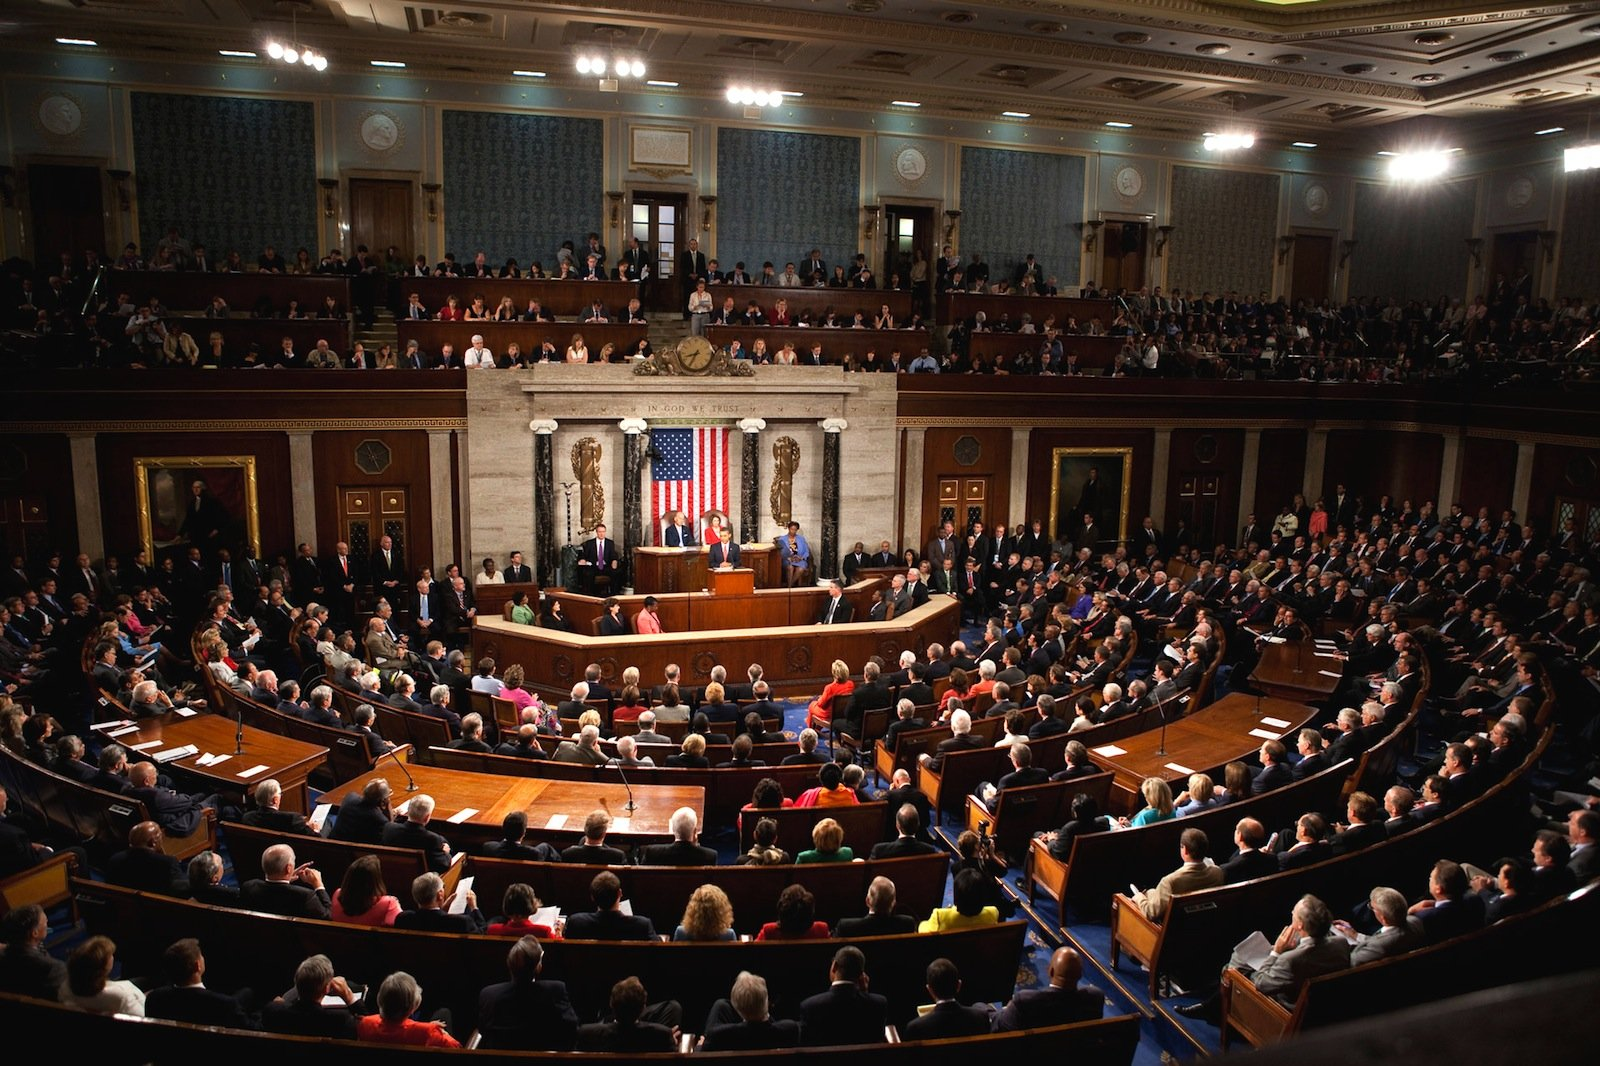
\includegraphics[width=\paperwidth,height=\paperheight]{images/interaction.jpg}}
  \begin{frame}
    \begin{textblock}{300}(0, 62)
    \begin{tikzpicture}
      \node [whitestripe] (stripe) {};
    \end{tikzpicture}
    \end{textblock}
    \begin{textblock}{300}(15,70)
      The study of interacting decision makers
    \end{textblock}
   \end{frame}
}
{
  \usebackgroundtemplate{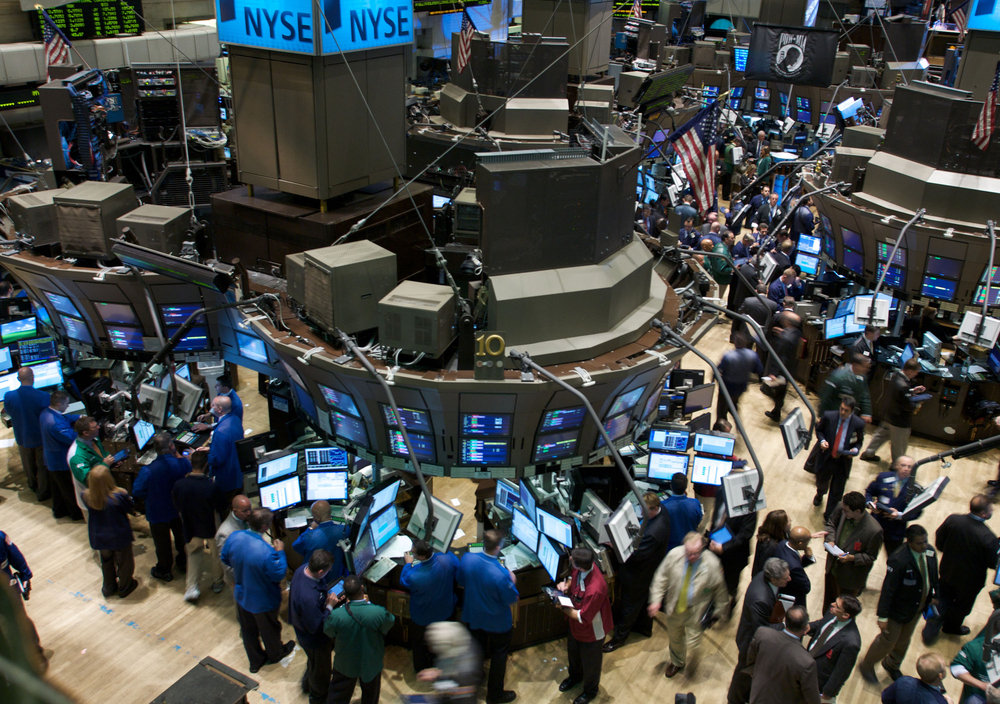
\includegraphics[width=\paperwidth,height=\paperheight]{images/wall_street.jpeg}}
  \setbeamercolor{normal text}{fg=red}
  \begin{frame}
    \begin{textblock}{300}(0, 102)
    \begin{tikzpicture}
      \node [whitestripe] (stripe) {};
    \end{tikzpicture}
    \end{textblock}
    \begin{textblock}{30}(170,110)
      Economy
    \end{textblock}
  \end{frame}
}

{
  \usebackgroundtemplate{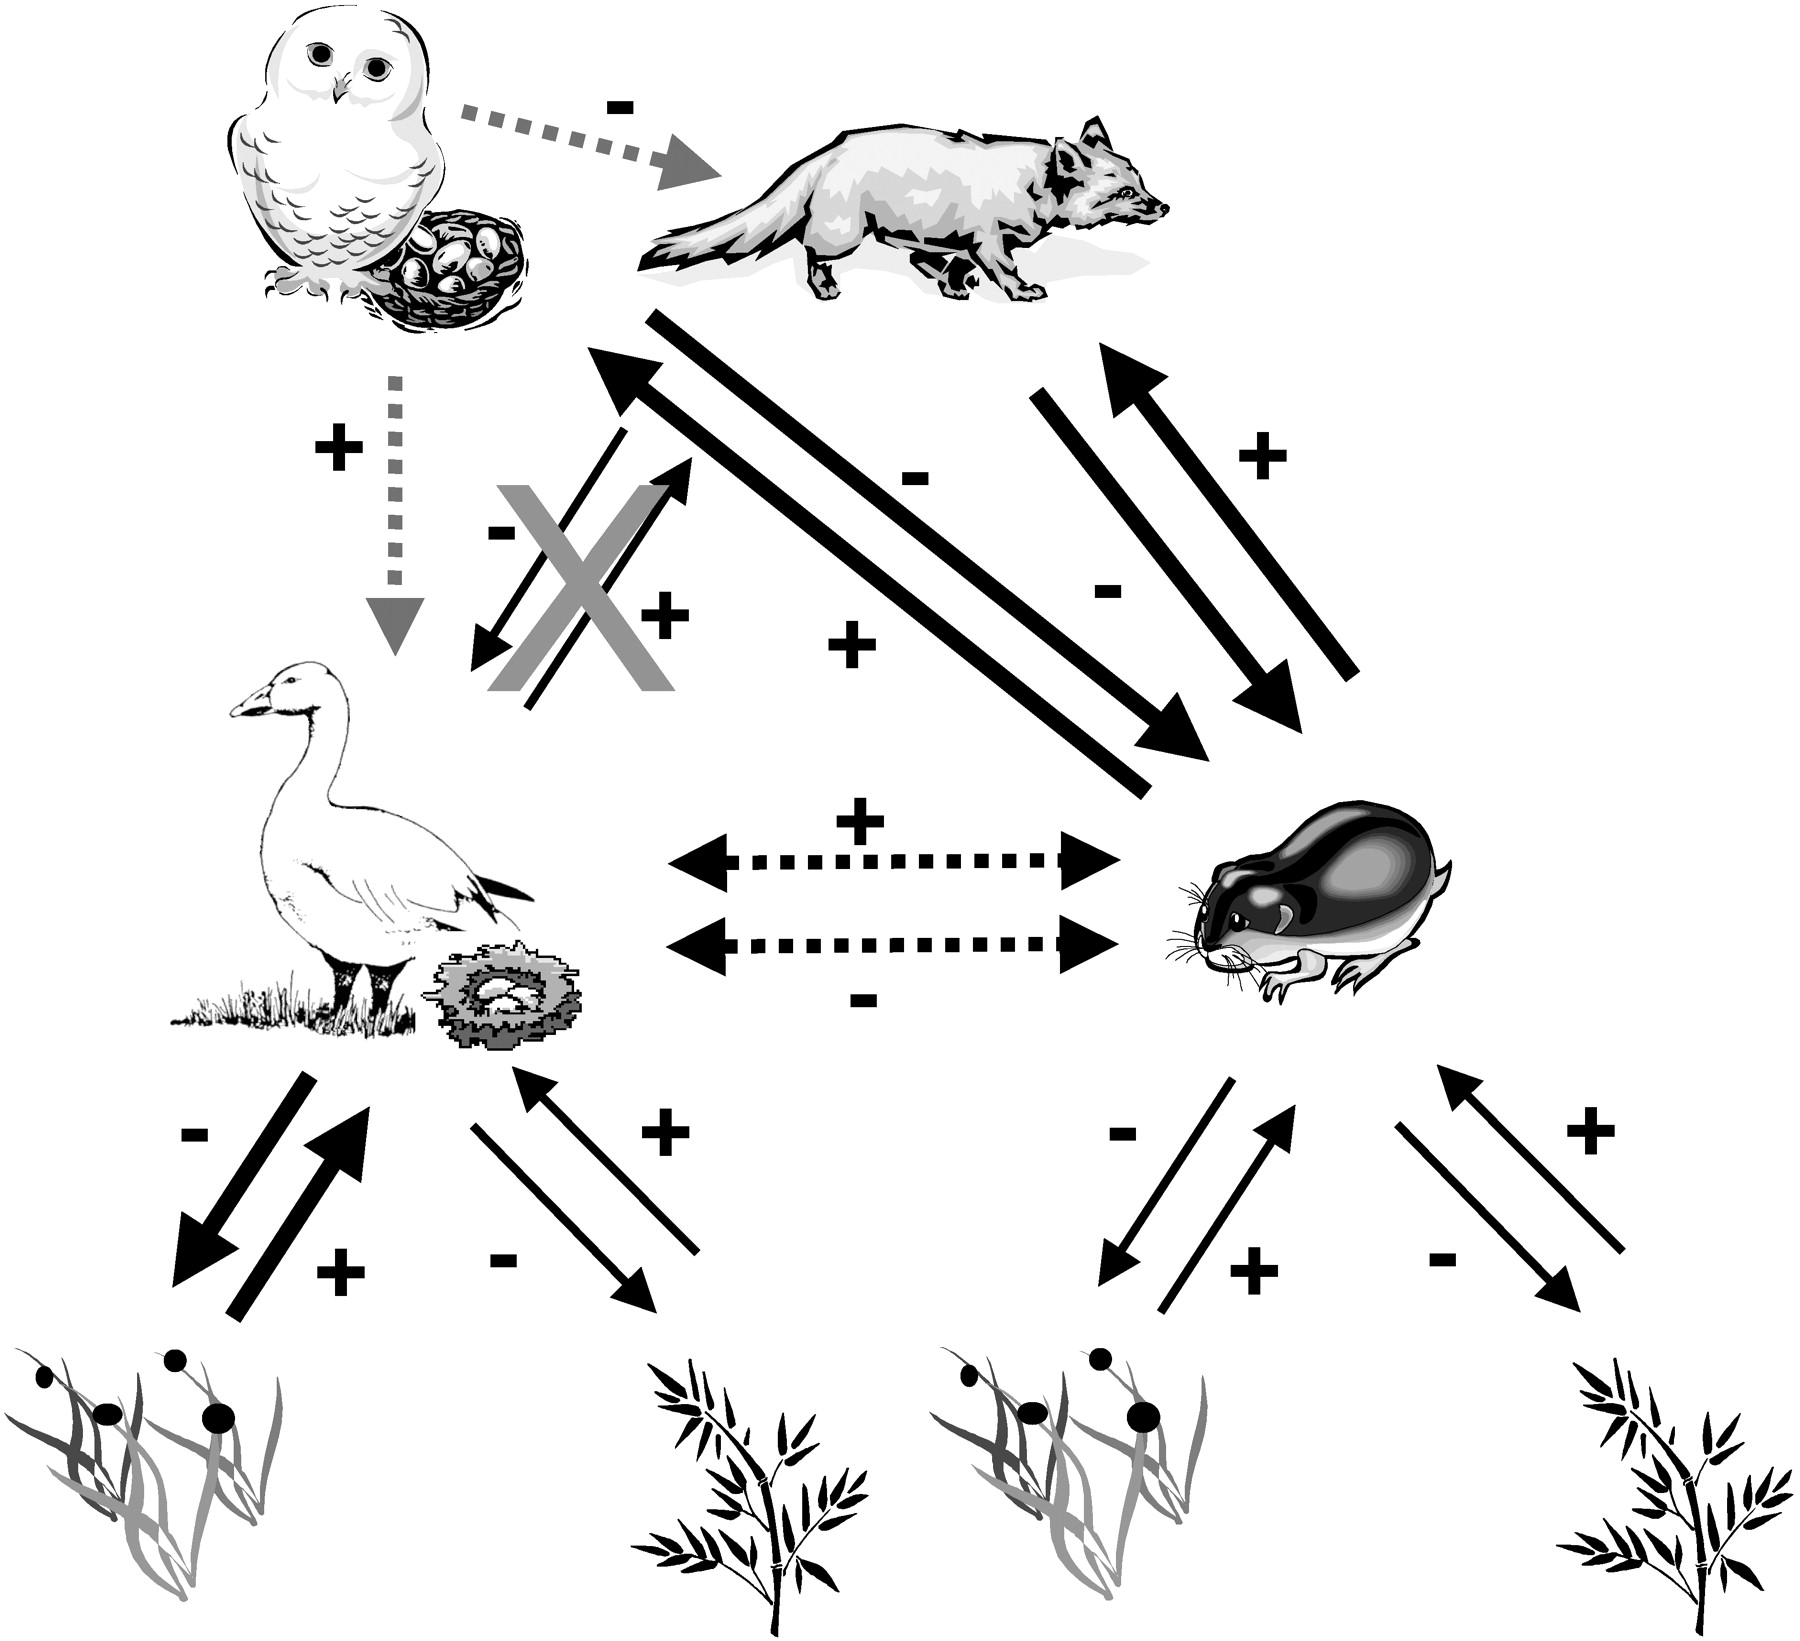
\includegraphics[width=\paperwidth, height=\paperheight]{images/biology.jpg}}
  \begin{frame}
    \begin{textblock}{30}(280,40)
      Biology
    \end{textblock}
  \end{frame}
}

{
  \usebackgroundtemplate{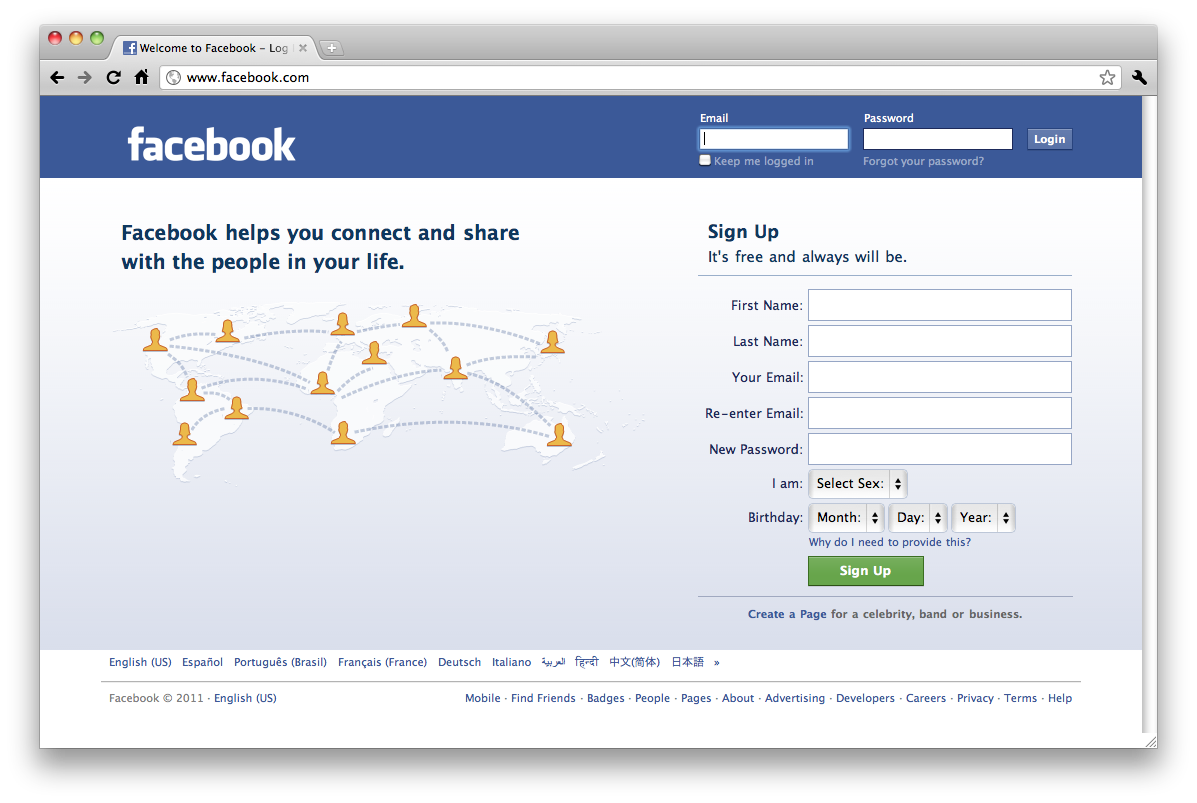
\includegraphics[width=\paperwidth, height=\paperheight]{images/facebook.png}}
  \begin{frame}
    \begin{textblock}{30}(80,180)
      Sociology
    \end{textblock}
  \end{frame}
}

{
  \usebackgroundtemplate{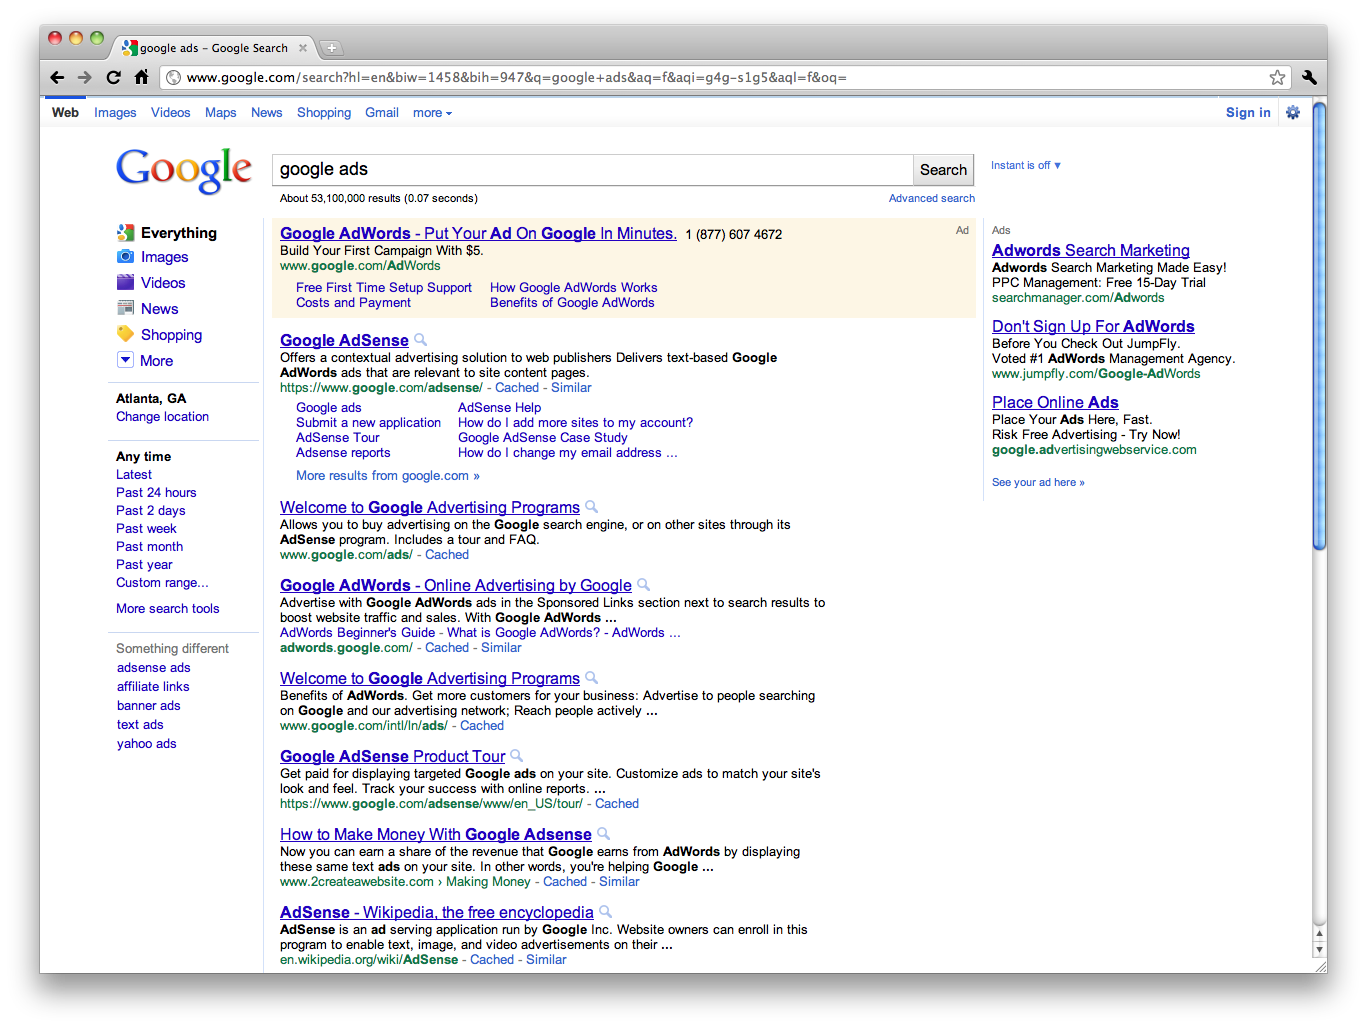
\includegraphics[width=\paperwidth, height=\paperheight]{images/google.png}}
  \begin{frame}
    \begin{textblock}{100}(250,180)
      Computer Science
    \end{textblock}
  \end{frame}
}

{
  \usebackgroundtemplate{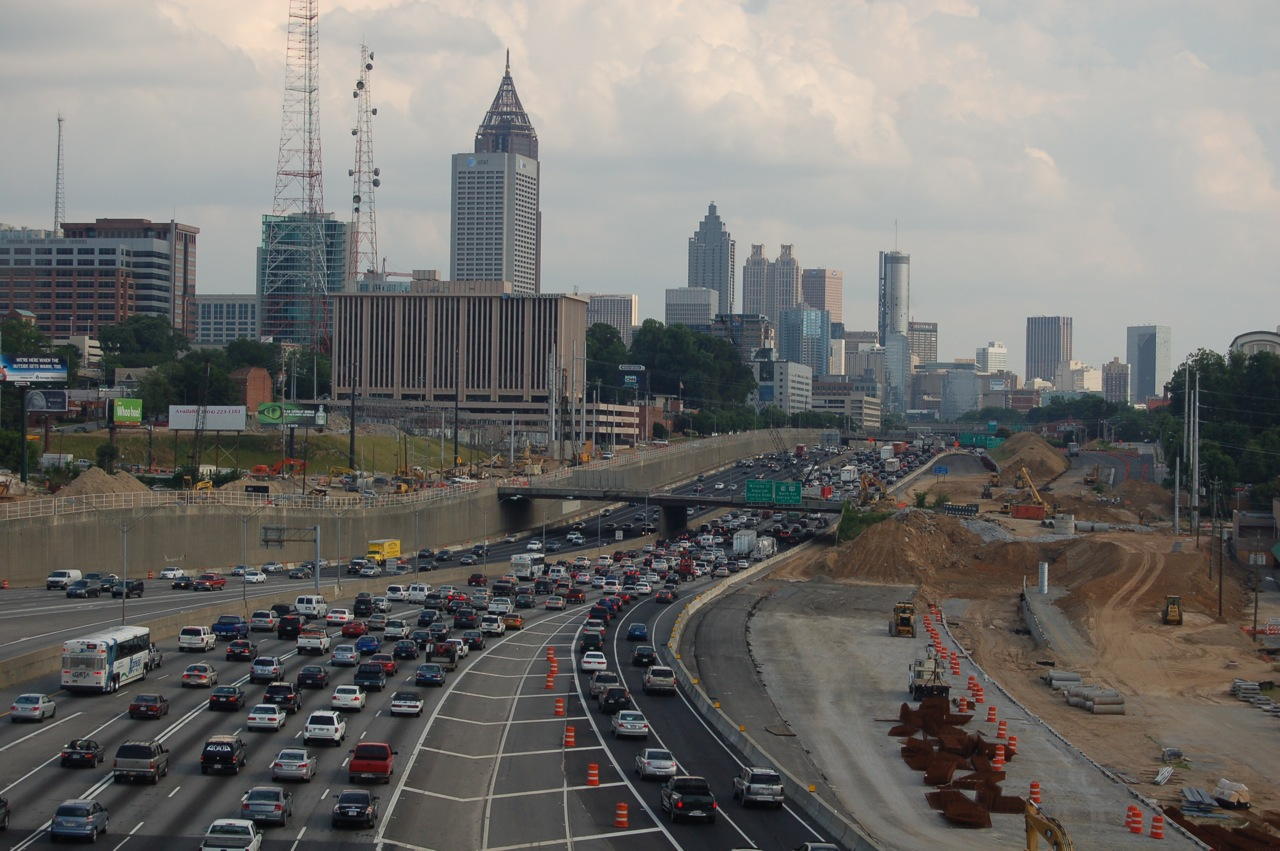
\includegraphics[width=\paperwidth, height=\paperheight]{images/congestion.jpg}}
  \begin{frame}
    \begin{textblock}{30}(230,30)
      Engineering
    \end{textblock}
  \end{frame}
}

{
  \usebackgroundtemplate{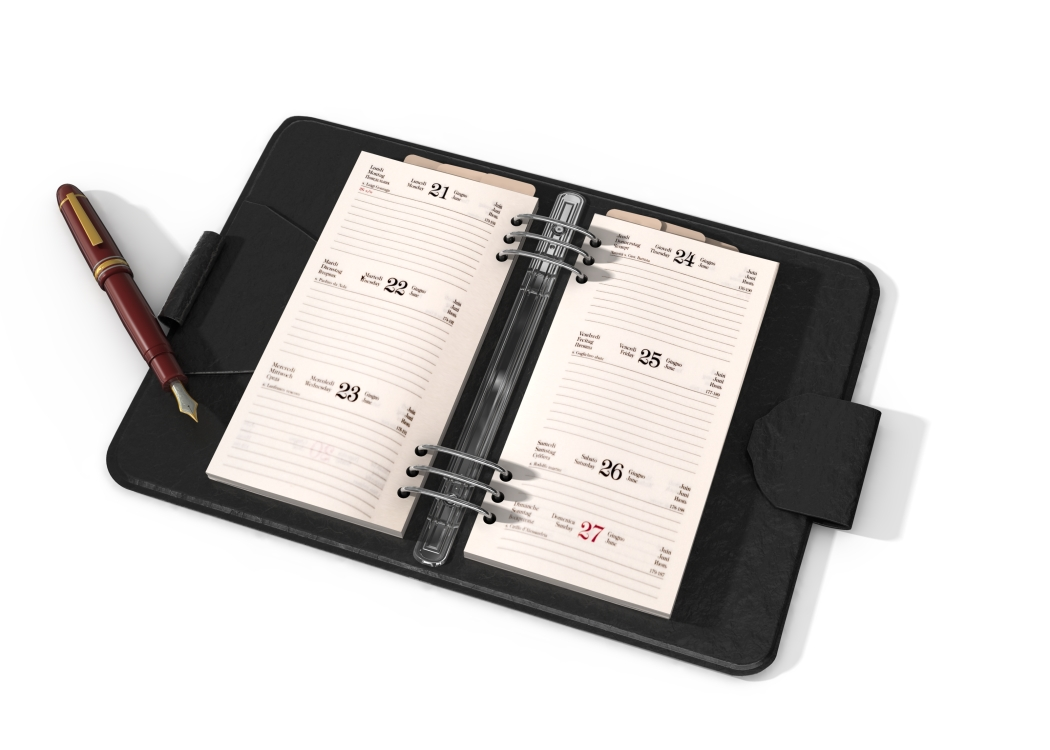
\includegraphics[width=\paperwidth, height=\paperheight]{images/agenda.jpg}}
  \begin{frame}
    \begin{textblock}{200}(200,30)
      Different agendas
    \end{textblock}
  \end{frame}
}


{
  \usebeamercolor[fg]{what how where}
  \setbeamercolor{background canvas}{bg=what how where.bg}
  \begin{frame}

    \frametitle{\textbf{What?}}
    \begin{itemize}
    \pause \item study of interacting decision makers
    \pause \item interdisciplinary field
    \pause \item different agendas
    \end{itemize}
  \end{frame}
}

\whw{How?}


\begin{frame}
  \frametitle{Decision maker}
  \begin{itemize}
  \item<2-> choices, $C$
  \item<3-> preferences, $\succeq$ \\
    \uncover<4>{utility function, $u:C \to \mathbb{R}$
    \[c_1 \succeq c_2 \iff u(c_1) \geq u(c_2)\]}
  \end{itemize}
\end{frame}

{
  \usebackgroundtemplate{
\includegraphics[width=\paperwidth, height=\paperheight]{images/decision_making.jpg}}
  \begin{frame}
    \begin{textblock}{30}(20,20)
    \uncover<2->{
      \[C = \{L,R\}\]}
    \end{textblock}

    \begin{textblock}{30}(10,160)
    \uncover<3->{
      \begin{eqnarray*}
        u:& C \to \mathbb{R}\\
        &L \mapsto 0\\
        &R \mapsto 1\\
      \end{eqnarray*}}
    \end{textblock}

    \begin{textblock}{30}(250,150)
    \uncover<4>{
      \begin{game}{2}{1}
            \> $u$ \\
        $L$ \>   $0$ \\
        $R$ \>   $1$
      \end{game}}
    \end{textblock}
  \end{frame}
  \note{explain the subscript i}
}

\begin{frame}

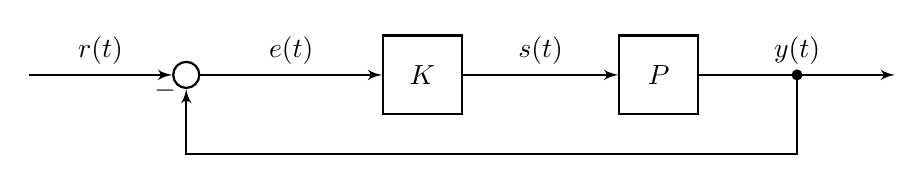
\begin{tikzpicture}[auto, node distance=3cm, >=latex', thick]
    % Placing the blocks
    \node [input, name=input] {};
    \node [sum, right of=input] (comparator) {};
    \node [block, right of=comparator] (controller) {$K$};
    \node [block, right of=controller] (plant) {$P$};
    \node [output, right of=plant] (output) {};
    \coordinate [below of=plant, node distance=1cm] (feedback);

    % Connecting the nodes
    \draw [->] (input) -- node {$r(t)$} (comparator);
    \draw [->] (comparator) -- node {$e(t)$} (controller);
    \draw [->] (controller) -- node {$s(t)$} (plant);
    \draw [->] (plant) -- node [coordinate, name=y, label=above:$y(t)$] {} (output);
    \draw [->] (y) |- (feedback) -| (comparator) node[pos=0.99] {$-$};

    \fill (y) circle (2pt);
\end{tikzpicture}


\bigskip

\pause
\begin{itemize}
\item<2-> $C = \{\text{stabilizing controller } K\}$
\item<3-> $u(K) = - \tau_r(K)$
\end{itemize}

\end{frame}

\begin{frame}
  \frametitle{Optimality}
  Decision maker:
  \begin{itemize}
  \item choices, $C$
  \item utility function, $u$
  \end{itemize}

  \bigskip

  \pause
  Goal of decision maker:
  \[\max_{c\in C} u(c)\]
\end{frame}

\begin{frame}
  \frametitle{Game Theory}

  \begin{itemize}
  \pause \item players, $\{i\}$
  \pause \item choices for player $i$, $C_i$
  \pause \item joint choices, $C=\prod_i C_i$\\
    $c\in C = (c_i, c_{-i})$
  \pause \item utility function for player $i$, $u_i:C \to \mathbb{R}$
  \end{itemize}
\end{frame}


\begin{frame}
  \frametitle{Optimality?}
  Goal of decision maker $i$:
  \[\max_{c \in C} u_i(c_i, c_{-i}) \left( \neq \max_{c \in C} u_i(c_i)
  \right)\]
\end{frame}

\begin{frame}
  \frametitle{Example: Prisoner's dilemma}

  \newcommand{\BR}{\text{BR}}

  \begin{game}{2}{2}
      \> \uncover<1-5,8->{$C$}    \>\uncover<1-2,6->{$D$} \\
  $C$ \>  $\uncover<1-5,8->{2}\uncover<1,8->{,2}$ \>$\uncover<1-2,6->{-1}\uncover<1,8->{,3$} \\
  $D$ \> $\uncover<1-5,8->{3}\uncover<1,8->{,-1}$ \>$\uncover<1-2,6->{0}\uncover<1,8->{,0$}
  \end{game}

  \bigskip
  \uncover<4->{Best response, $\BR_i: C_{-i} \rightrightarrows C_i$}
  \begin{itemize}
  \item<5-> $\uncover<5->{\BR_1(C) = \{D\}}  \uncover<7->{, \BR_1(D) = \{D\}}$
  \item<9-> $\uncover<9->{\BR_2(C) = \{D\}, \BR_2(D) = \{D\}}$
  \end{itemize}

\end{frame}

\begin{frame}
  \frametitle{Nash equilibrium}
  $a^* = (a_i^*, a_{-i}^*)$ is a Nash equilibrium:
  \begin{itemize}
  \pause \item $\forall i$, $a_i^*$ is a best response to $a_{-i}^*$
  \pause \item no unilateral deviation is profitable
  \pause \item  $\forall i$, $\forall a_i \in A_i$,
    \[u_i(a_i^*, a_{-i}^*) \geq u_i(a_i, a_{-i}^*)\]
  \end{itemize}
\end{frame}

\begin{frame}
  \frametitle{Existence of Nash equilibria}

  Every $n$-player game has a Nash equilibrium.
\end{frame}

\begin{frame}
  \frametitle{Extensions}
  \begin{itemize}
  \pause \item history-dependent strategy
  \pause \item imperfect information
  \pause \item cooperation
  \pause \item large populations
  \end{itemize}
\end{frame}

\begin{frame}
  \frametitle{Back to the agendas}
  \begin{itemize}
  \pause \item descriptive
  \pause \item predictive
  \pause \item manipulative
  \end{itemize}
\end{frame}

{
  \usebeamercolor[fg]{what how where}
  \setbeamercolor{background canvas}{bg=what how where.bg}
  \begin{frame}

    \frametitle{\textbf{How?}}
    \begin{itemize}
    \pause \item interacting decision maker
    \pause \item best response
    \pause \item Nash equilibrium
    \end{itemize}
  \end{frame}
}

\whw{Where?}

\begin{frame}
  \frametitle{Learning}
  Controls $\Rightarrow$ Game Theory:
  \begin{itemize}
  \pause \item stability and robustness
  \pause \item derivative control
  \end{itemize}
  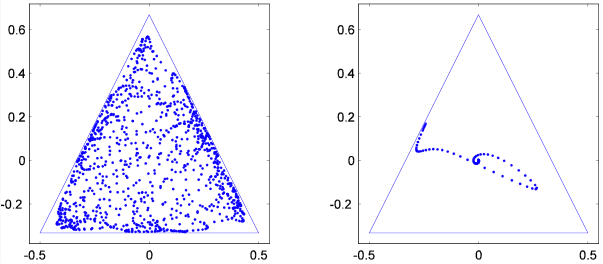
\includegraphics[width=0.6\paperwidth]{images/derivative_control.png}
\end{frame}

\begin{frame}
  \frametitle{Decentralized control}
  Game Theory $\Rightarrow$ Controls:
  \begin{itemize}
  \pause \item network formation
  \pause \item communication limitations
  \end{itemize}
\end{frame}

\begin{frame}
  \frametitle{Dynamic Games}
  \begin{itemize}
  \pause \item network security
  \pause \item learning in repeated games
  \end{itemize}
\end{frame}

{
  \usebeamercolor[fg]{what how where}
  \setbeamercolor{background canvas}{bg=what how where.bg}
  \begin{frame}

    \frametitle{\textbf{Where?}}
    \begin{itemize}
    \pause \item learning
    \pause \item decentralized control
    \pause \item dynamic games
    \end{itemize}
  \end{frame}
}


{
  \usebeamercolor[fg]{what how where}
  \setbeamercolor{background canvas}{bg=what how where.bg}
  \begin{frame}

    {\Huge Questions? \\ \bigskip \bigskip Comments?}
  \end{frame}
}


\end{document}
